\documentclass{beamer}
\usepackage[utf8]{inputenc}
\usepackage[squaren]{SIunits}
\usepackage{varwidth,setspace}
\usepackage{tikz}
\usetikzlibrary{intersections,positioning,backgrounds,fit,matrix,shapes,calc,decorations.pathmorphing,decorations.text}
\usetheme{default}

\newcommand*{\mimg}[2]{\begingroup
\setbox0=\hbox{\includegraphics[height=#2]{#1}}\parbox{\wd0}{\box0}\endgroup}
\newcommand*{\rmimg}[2]{\begingroup
\setbox0=\hbox{\includegraphics[angle=90,origin=c,height=#2]{#1}}\parbox{\wd0}{\box0}\endgroup}
\newcommand*{\symok}[0]{\includegraphics[height=1em]{symbol_ok.pdf}}
\newcommand*{\symbad}[0]{\includegraphics[height=1em]{symbol_bad.pdf}}
\newcommand*{\symidk}[0]{{\bf\color{blue}\Large?}}

\setbeamertemplate{navigation symbols}{}%remove navigation symbols
\setbeamertemplate{footline}{\hspace*{.5cm}\scriptsize{\hfill\raisebox{1mm}{\insertframenumber}\hspace*{.5cm}}}

\setlength{\tabcolsep}{0.5mm}

\title{Exploring the dark universe with the Atacama Cosmology Telescope}
\author{Sigurd Kirkevold Næss}
\institute{Subdepartment of astrophysics, Oxford University}
\date{October 13th, 2014}

\begin{document}

\begin{frame}
	\titlepage
	\vspace{-1cm}
	\begin{center}
	%{\footnotesize The source code of this talk can be found at {\color[rgb]{0,0.7,0}https://github.com/amaurea/talk-bmode}}
	\end{center}
\end{frame}

\begin{frame}{The physics of CMB lensing}
\end{frame}

\begin{frame}{Lensing distorts the CMB}
	\begin{center}
		\only<1>{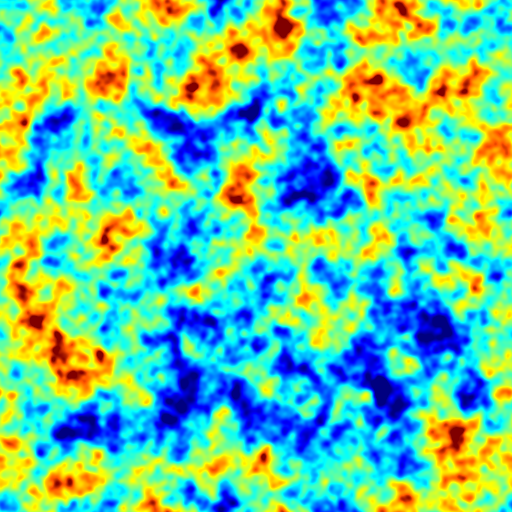
\includegraphics[height=7cm]{plots/maps/T.png}}%
		\only<2>{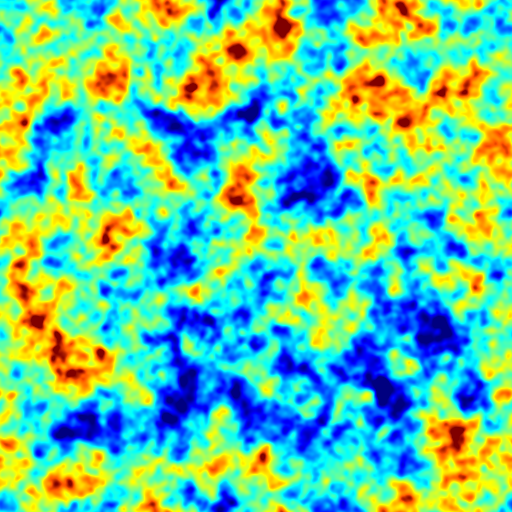
\includegraphics[height=7cm]{plots/maps/TlT.png}}%
		\only<3-4>{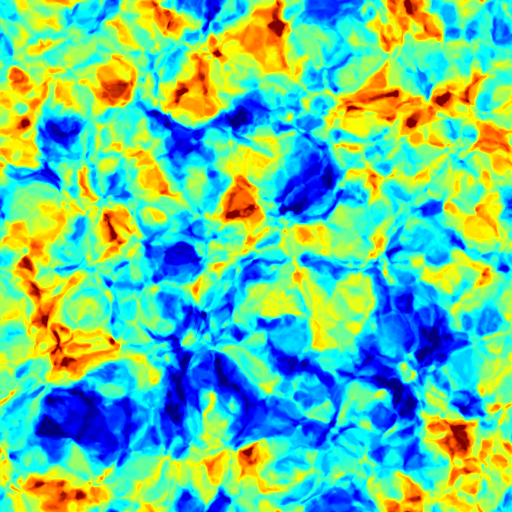
\includegraphics[height=7cm]{plots/maps/TsT.png}}%

		\only<1>{Unlensed}%
		\only<2>{Lensed}%
		\only<3>{Lensed x10}%
		\only<4>{Non-Gaussian}%
	\end{center}
\end{frame}

\begin{frame}{Lensing distorts the CMB Polarization}
	\begin{center}
		\hspace*{-3mm}
		\begin{tabular}{cc}
			{\bf Q} ($\pm 20\mu$K) & {\bf U} ($\pm 20\mu$K) \\
			\only<1>{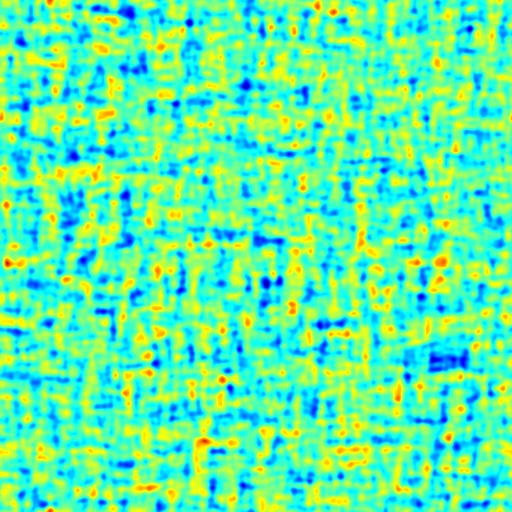
\includegraphics[height=5.5cm]{plots/maps/EBQ.png}}%
			\only<2>{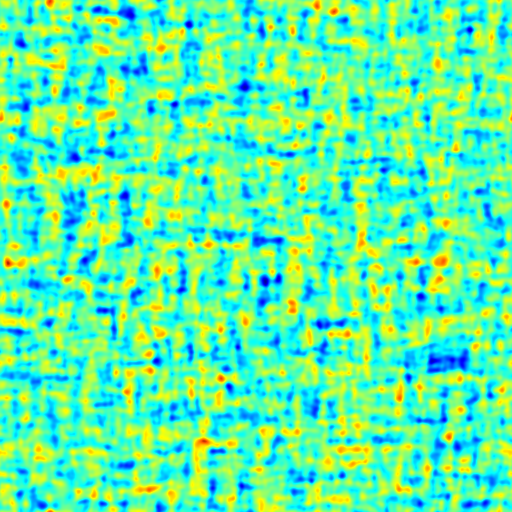
\includegraphics[height=5.5cm]{plots/maps/EBlQ.png}}%
			&
			\only<1>{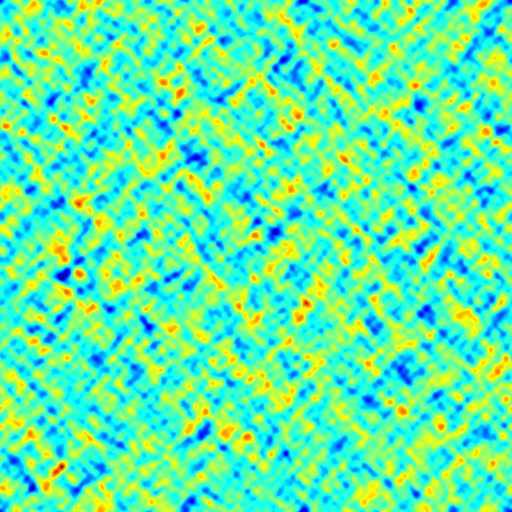
\includegraphics[height=5.5cm]{plots/maps/EBU.png}}%
			\only<2>{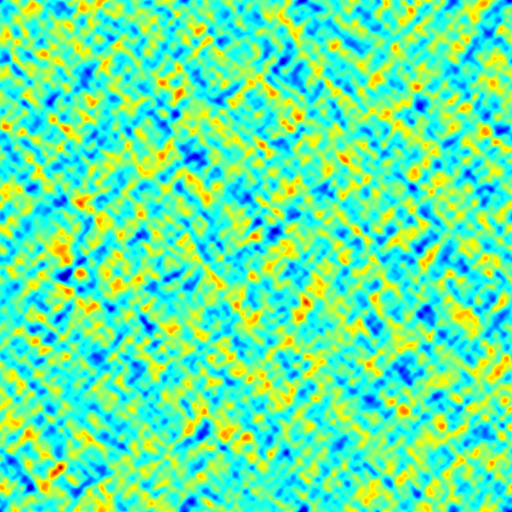
\includegraphics[height=5.5cm]{plots/maps/EBlU.png}}%
		\end{tabular}

		\only<1>{Unlensed}%
		\only<2>{Lensed}%
	\end{center}
\end{frame}

\begin{frame}{E, B and Q, U}
	\begin{center}
		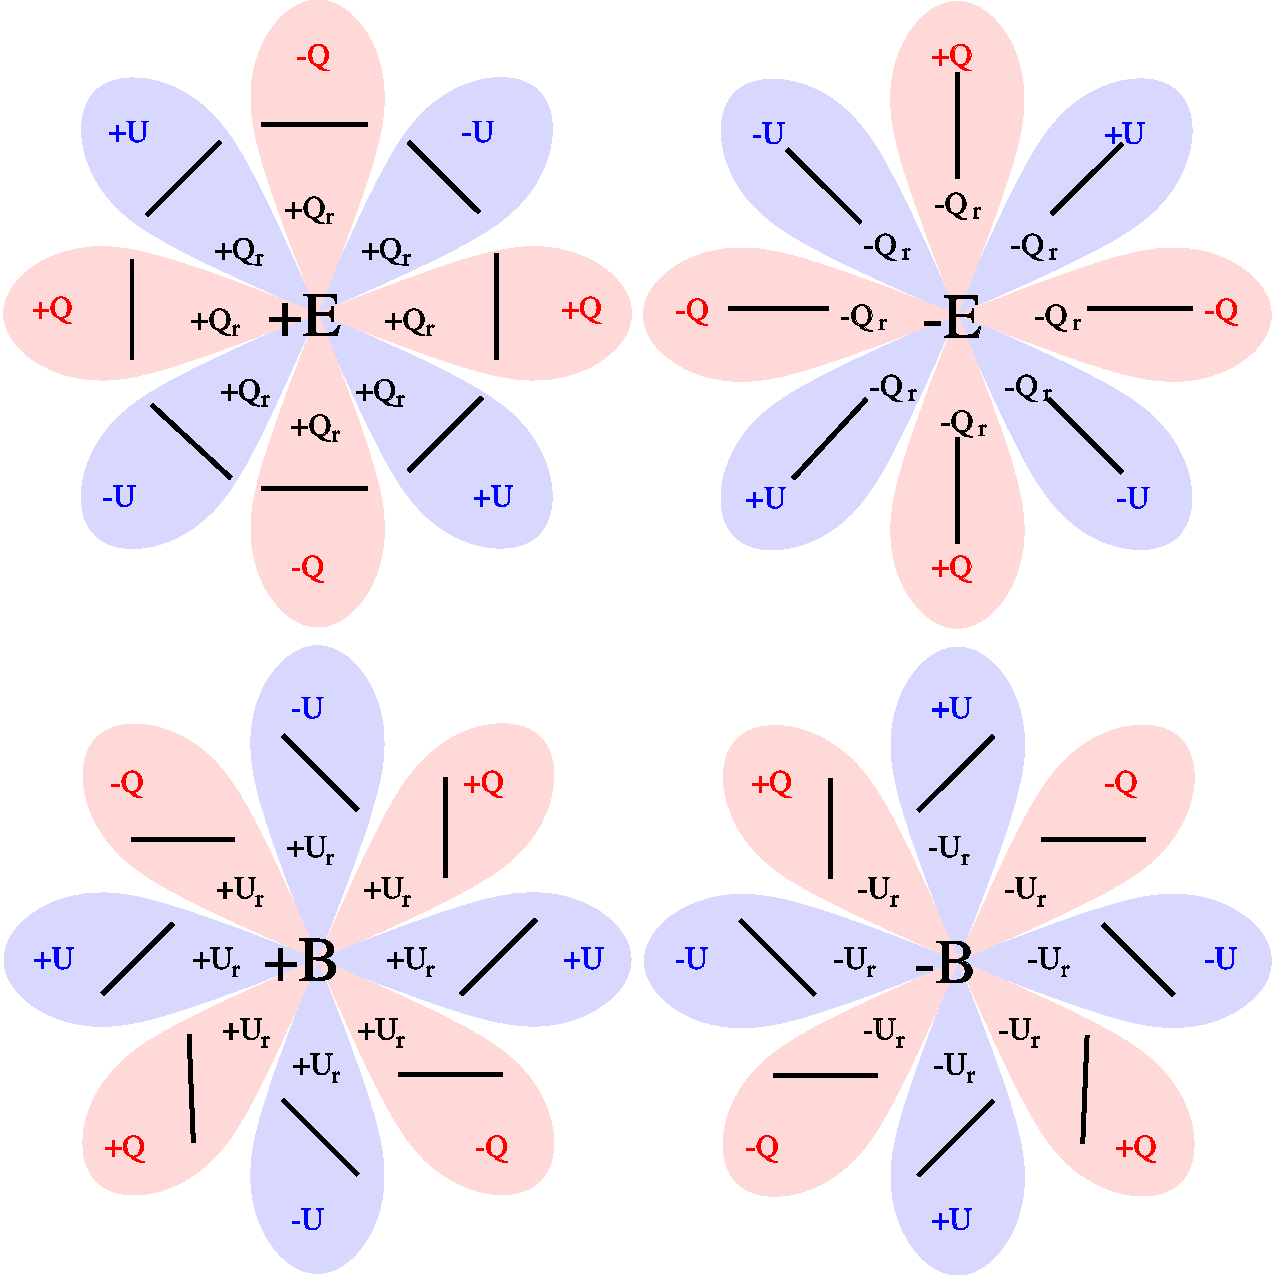
\includegraphics[height=8cm]{plots/EB_healpix.pdf}
	\end{center}
\end{frame}

\begin{frame}{E,B and Q, U}
	\begin{center}
		\only<1>{E and B result from quadrupole-convolutions of Q and U}%
		\only<2>{Reverse also holds}%

	\scalebox{1.7}{
		\begin{minipage}{5cm}
			\begin{align*}
				\only<1>{%
				E =& \rmimg{plots/queb_0.png}{1cm} \otimes Q + \mimg{plots/queb_2.png}{1cm} \otimes U \\
				B =& \mimg{plots/queb_1.png}{1cm} \otimes Q + \rmimg{plots/queb_3.png}{1cm} \otimes U}%
				\only<2>{%
				Q =& \rmimg{plots/ebqu_0.png}{1cm} \otimes E + \mimg{plots/ebqu_2.png}{1cm} \otimes B \\
				U =& \mimg{plots/ebqu_1.png}{1cm} \otimes E + \rmimg{plots/ebqu_3.png}{1cm} \otimes B}%
			\end{align*}
		\end{minipage}}
	\end{center}
\end{frame}

\begin{frame}{Lensing distorts E and B}
	\begin{center}
		\hspace*{-3mm}
		\begin{tabular}{cc}
			{\bf E} ($\pm 20\mu$K) & {\bf B} ($\pm 0.5\mu$K) \\
			\only<1>{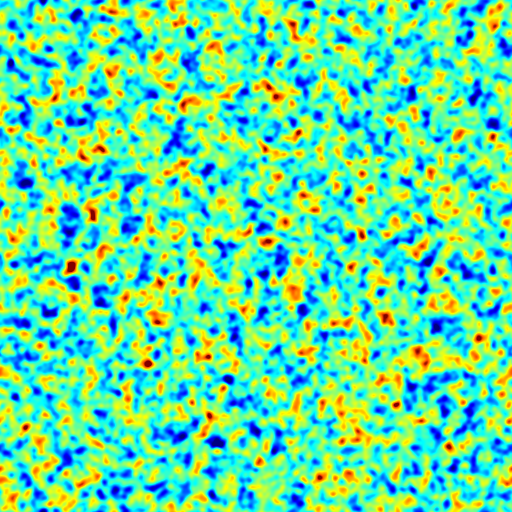
\includegraphics[height=5.5cm]{plots/maps/E.png}}%
			\only<2>{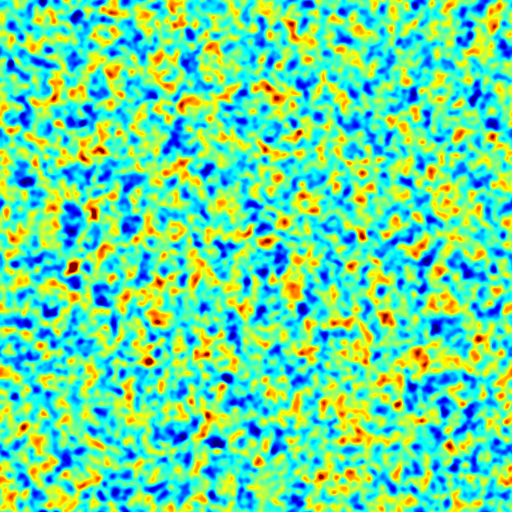
\includegraphics[height=5.5cm]{plots/maps/EBlE.png}}%
			&
			\only<1>{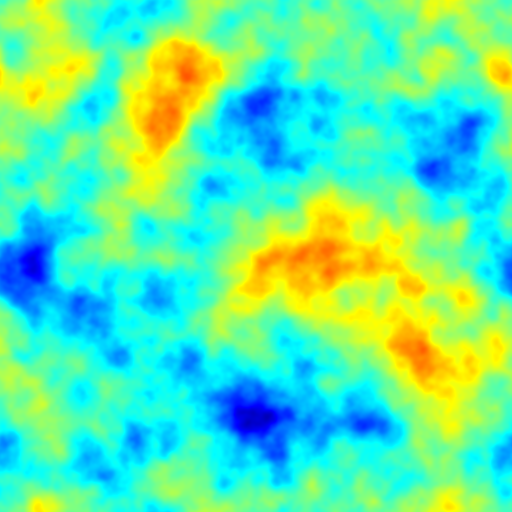
\includegraphics[height=5.5cm]{plots/maps/B.png}}%
			\only<2>{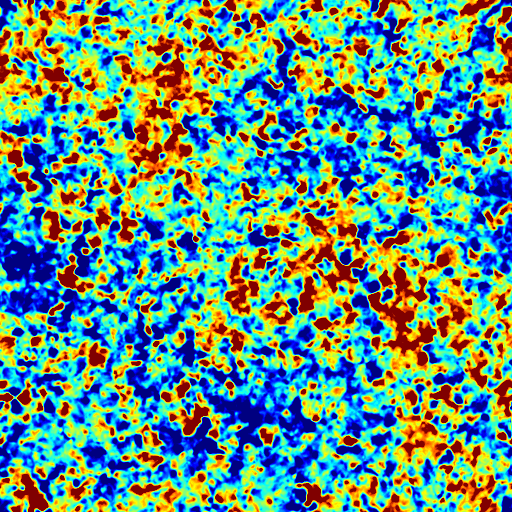
\includegraphics[height=5.5cm]{plots/maps/EBlB.png}}%
		\end{tabular}

		\only<1>{Unlensed}%
		\only<2>{Lensed}%
	\end{center}
\end{frame}

\begin{frame}{Disentangling CMB and lensing}
\end{frame}

\begin{frame}{Lensing as an observable}
\end{frame}

\begin{frame}{Good systematics}
\end{frame}

\begin{frame}{Observational status}
\end{frame}

\begin{frame}{(Near) future}
\end{frame}

\end{document}
